\documentclass[handout]{beamer}
\usepackage[utf8]{inputenc}

\usepackage{natbib}  %havard referencing
\bibliographystyle{agsm}
\usepackage{xcolor}
\usepackage[tikz]{bclogo}
\usepackage[framemethod=tikz]{mdframed}
\usepackage{lipsum}
\usepackage{tikz,lipsum,lmodern}
\usepackage[most]{tcolorbox}
\usepackage{caption}
\usepackage{etoolbox}
\AtBeginDocument{\patchcmd{\label}{\strut}{}{}{}}
\usepackage{amsmath}
\usepackage{amssymb}
\usepackage[ruled,vlined]{algorithm2e}
\usepackage{amsthm}
\usepackage{amsfonts}
\usepackage{graphicx}
\usepackage{amsmath}
\usepackage{amssymb}
\usepackage{amsthm}
\usepackage{amsfonts}
\usepackage{xspace}
\usepackage{mathtools}
\usepackage[noend]{algpseudocode}
\usepackage{color}
\usepackage{tikz}
\usetikzlibrary{arrows}
\usepackage{xmpmulti}

\mode<presentation>
{
  \usetheme{Madrid}      % or try Darmstadt, Madrid, Warsaw, ...
  \usecolortheme{default} % or try albatross, beaver, crane, ...
  \usefonttheme{default}  % or try serif, structurebold, ...
  \setbeamertemplate{navigation symbols}{}
  \setbeamertemplate{caption}[numbered]
} 

\usepackage[english]{babel}
\title[Mobile Ticket Inspection on ICEs]{Mobile Ticket Inspection on ICEs}
\author[May, Nguyen \& Abrams]{Nathan May \inst{1} \and Hai Nguyen \inst{2} \and 
Ruby Abrams \inst{3}}
\institute[]{\inst{1} Department of Mathematics, Washington State University, U.S.A. \and %
             \inst{2} School of Computer Science, University of Birmingham, U.K. \and
             \inst{3} Department of Mathematics, University of Arizona, U.S.A.}
                      
%\author[May, Nguyen \& Abrams]{Nathan May, Hai Nguyen \& Ruby Abrams}
%\institute[ZIB]{Zuse Institut Berlin\\
%Berlin, Germany}

\date[Transportation Seminar]{Transportation Seminar\\
July 23, 2019}

\begin{document}

\begin{frame}
  \titlepage
\end{frame}

\begin{frame}{Outline}
\small 
  \tableofcontents
\end{frame}

\section{The Inspector Scheduling Problem}

\begin{frame}{The Inspector Scheduling Problem}
\textbf{Input:}

\begin{itemize}
    \item Number of inspectors 
    \item Depot station for each inspector (also called base)
    \item Maximum number of working hours for each inspector
    \item Train timetable \& train statistics for a specific day
\end{itemize}

\textbf{Output:}

A day-long working schedule for each inspector 
in order to maximise the number of passengers inspected 
on that day.
\end{frame}

\section{A Brief Literature Review}

\begin{frame}{Related Work}

Previous studies have considered a \textbf{game-theoretic approach}.

\begin{itemize}
    %\item Stackelberg strategies
    \item Leader (ticket inspector) vs. Follower (fare evader)
    \item First considered in 
    \cite{yin_jiang_tambe_kiekintveld_leyton-brown_sandholm_sullivan_2012} for the 
    LA transit systems (formulated as a bi-level programming problem)
    \item \cite{jiang_yin_johnson_tambe_kiekintveld_leyton-brown_sandholm_2012} improved \cite{yin_jiang_tambe_kiekintveld_leyton-brown_sandholm_sullivan_2012} 
    upon \textit{history encoding} and 
        \textit{schedule regularisation} 
  
    %\item In \cite{jiang_yin_johnson_tambe_kiekintveld_leyton-brown_sandholm_2012}, optimal scheduling %model TRUSTS implements temporal and spatial constraints to defer \textit{fare evasion} and maximise %revenue in the form of a Stackelberg strategy (in our case, maximise number of inspected passengers).
\end{itemize}

\textbf{Our remarks}: 
\begin{itemize}
    \item We try to maximise the number of passengers inspected
    \item We do not take into account fare evaders
\end{itemize}
\end{frame}

\section{Our Approach}

\begin{frame}{How do we approach the problem?}
\begin{enumerate}
    \item Formulate the  Inspector Scheduling problem as a Network Flow Problem
    \item Estimate Origin-Destination (OD) Matrices 
    in order to maximise the number of people inspected on all trips
    \item Solve our network flow as a Mixed Integer Programming (MIP)
\end{enumerate}
\end{frame}

\subsection{Network Representation}

\begin{frame}{Network Representation}
\begin{figure}
    \centering
    \begin{subfigure}
        \includegraphics[scale=0.13]{graph__.png}
     \end{subfigure}
    %\caption{\small A transition graph (Krogvig, %2014). There are 5 stations; 
    %each is represented by a line. The x-axis %represents time.
    %Each dot is an event, defined by "a train departs %from or arrives at a station". Cyan arrows are %driving arcs, while grey arrows are waiting arcs.}
\end{figure}
\end{frame}

\begin{frame}{Model Parameters (Input)}
    %\underline{Parameters (Input):}\\
    \begin{itemize}
        \item $K$ inspectors working
        \item $\theta_k$ - number of hours inspector k is allowed to work
        \item For every edge $e := (A_{t_1}, B_{t_2})$ from stations $A$ to $B$:
        \begin{enumerate}
            \item $t_e = t_1 - t_2$, the trip time
            \item $v_e$, the number of passengers on train $e$
        \end{enumerate}
        %\item $t_{(A,B)}$ - time it takes for a %train to travel from station $A$ to %station $B$
        %\item $v_{(A_{t_1}, B_{t_2})}$ - number of %people travelling on a train from stations %$A$ to $B$, at times $t_1$ and $t_2$
        \item $r$ - inspection rate (constant for all inspectors)
        \item $\Lambda \subset \mathcal{P}(\Omega)$, set of origin-destination passenger trips ($\Omega$ - set of all trains)
        \item $T_{\lambda}$ - number of people taking trip $\lambda \in \Lambda$
        \item $f_e = \frac{r\cdot t_e}{v_e}$ - inspector effectiveness on an edge $e$
    
    \end{itemize}
\end{frame}

\begin{frame}{Variables (Output)}
    %\underline{Variables (Output):}\\
    \begin{itemize}
        \item $x^{(k)}_{e}$ - decision variable, whether or not inspector $k$ takes train $e$
        \item $M_{\lambda}$ - dummy variable, for reconstructing a minimum in the objective function (percentage of people taking path $\lambda$ that have been inspected)
        
    \end{itemize}
    \begin{figure}
        \centering
        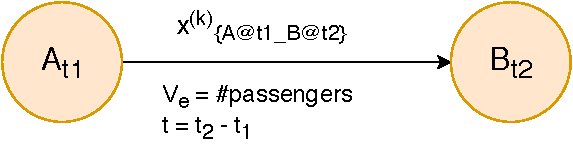
\includegraphics[scale=0.7]{nodes.pdf}
        \caption{Description of an edge between nodes and properties associated to each}
    \end{figure}

\end{frame}

\subsection{Probability of Passenger Inspection}

\begin{frame}{Probability of Passenger Inspection}
\begin{itemize}
    \item We classify passengers according to their trajectories (time of departure, origin station, destination station). 
    
    \item The \textbf{probability that a passenger of type $\lambda$ is inspected} by an inspector is
\begin{align*}
    \min\bigg\{1,\sum_{i=1}^K\sum_{e\in P_i\cap\lambda} f_e\bigg\}
\end{align*}
where:
\begin{itemize}
    \item $f_e$ -- \textit{inspector effectiveness} value assigned to edge $e$
    \item $P_i$ -- the patrol strategy for the $i^{th}$ inspector
    \item $\lambda$ -- a particular path taken by a passenger
\end{itemize}
\end{itemize}

\end{frame}

\begin{frame}{Objective Function Formulation}
   \textbf{Maximise} the number of inspected passengers of each type.
    \begin{align*}
        \max\sum_{\lambda\in \Lambda}T_{\lambda}\cdot\min\bigg\{1,\sum_{e\in\lambda}f_e\bigg(
            \sum_{i=1}^K x_{e}^{i}
        \bigg)\bigg\}
    \end{align*}
    
    % Issue: how do we determine the number of passengers of each type, $T_\lambda$?

\end{frame}

% \begin{frame}{Standard Network Flow Constraints}
%     mass-balance
%     \begin{align*}
%         \sum\limits_{p \in N^*}x^{(k)}_{(p,q)} - \sum\limits_{p \in N^*}x^{(k)}_{(q,p)} =0,\  \ \forall\ q \in N,\ k \in K
%     \end{align*}
%     flow into sinks and out of sources
%     \begin{align*}
%         \sum\limits_{(S_k,p) \in A^{(k)}}x^{(k)}_{(S_k,p)} = \sum\limits_{(p,T_k) \in A^{(k)}}x^{(k)}	_{(p,T_k)} = 1,\ \forall k \in K
%     \end{align*}
% \end{frame}

% \begin{frame}{Time Flow Constraint}
% time-flow constraint for each inspector
%     \begin{align*}
%         \sum\limits_{(A,T_k) \in A^{(k)}}x^{(k)}	_{(A,T_k)}t^{(k)}_{(A,T_k)} - \sum\limits_{(S_k,A) \in A^{(k)}}x^{(k)}_{(S_k,A)}t^{(k)}_{(S_k,A)} \leq \theta_k,\ \forall k \in K
%     \end{align*}
% \end{frame}

\section{Mixed Integer Programming Formulation}

\begin{frame}{MIP Formulation}

$$\textbf{maximise}\ \sum\limits_{\lambda \in \Lambda}T_{\lambda} \cdot M_{\lambda}$$
Subject to:

\begin{align}
	&\sum\limits_{A \in N^*}x^{(k)}_{(A,B)} - \sum\limits_{A \in N^*}x^{(k)}_{(B,A)} =0,\  \ \forall\ B \in N^* \setminus N,\ k \in K\\
	&\sum\limits_{(S_k,A) \in A^{(k)}}x^{(k)}_{(S_k,A)} = \sum\limits_{(A,T_k) \in A^{(k)}}x^{(k)}	_{(A,T_k)} = 1,\ \forall k \in K\\
	&\sum\limits_{(A,T_k) \in A^{(k)}}x^{(k)}	_{(A,T_k)}t^{(k)}_{(A,T_k)} - \sum\limits_{(S_k,A) \in A^{(k)}}x^{(k)}_{(S_k,A)}t^{(k)}_{(S_k,A)} \leq \theta_k,\ \forall k \in K\\
	&M_{\lambda} \leq 1,\ \forall \lambda \in \Lambda,\ \
	M_{\lambda} \leq \sum\limits_{e \in \lambda,\ k \in K}f_e \cdot x^{(k)}_{e},\ \forall \lambda \in \Lambda\\
	&x^{(k)}_{e} \in \mathbb{Z}_2,\  M_{\lambda} \in \mathbb{R}
\end{align}
\end{frame}

% \begin{frame}{Assumptions and Simplifications}
% \textbf{Assumptions:}
%     \begin{itemize}
%         \item We assume that every inspector inspects at the same rate. (used in calculating the edge effectiveness)
%         \item More than one inspector are allowed on each train ride.
%         \item All paths taken are the shortest driving paths.
%     \end{itemize}
% \textbf{Simplifications:}
%     \begin{itemize}
%         \item Data suggests that multiple trains can travel between two nodes. We can accommodate for this case, but assume that every edge is unique.
%         \begin{itemize}
%             \item We can store multiple edges using a Multi-DiGraph structure.
%             \item We need to account for multiple shortest paths in the OD Matrix (modify the multi-proportional algorithm). 
%         \end{itemize}
%     \end{itemize}
% \end{frame}

% \begin{frame}{Estimating Origin-Destination Matrix}
% \begin{itemize}
%     \item To avoid re-inspection of passengers on trains for several stops
%     \item First proposed by \cite{van_zuylen_willumsen_2002} which requires no priori knowledge.
%     \item Various approaches: information minimising/entropy maximisation
%     \item  \textbf{Input}: Directed graph with link volumes (i.e., number of passengers on board)
%      \item \textbf{Output}: Entry $(i,j)$ of the OD matrix representing the 
%      approximate number of passengers travelling from node $i$ to node $j$.
% \end{itemize}

% \end{frame}

\begin{frame}{Challenges}

    \textbf{Lack of individual passenger data:}\vspace{5mm}

    While we are able to estimate passenger data, we lack any 'a-priori' passenger data that's is often helpful in estimation.
\end{frame}

\begin{frame}{Future Work}
    \begin{itemize}
        \item Obtaining realistic results
        \item Complexity analysis
    \end{itemize}
\end{frame}






% \begin{frame}{New/Added Assumptions}
%     \textbf{Assumptions:}

%     \begin{itemize}
%         \item Multiple inspectors can inspect the same train
        
%         % \item Entirely new people get on the train every stop (subject of further study)
        
%         \item Inspectors do not get any scheduled breaks
        
%         \item The number of people taking a train remains the same for that day of the week
%     \end{itemize}
%     \begin{itemize}
%         \item All inspectors inspect at the same rate
%         \item All paths taken are the shortest paths
%         \item For simplicity: travel edges between events are unique 
%         \begin{itemize}
%             \item We do not account for multiple separate trains doing the same trip. However, we know how to and how to modify our own code.
%             \item O-D matrix accounts for all paths (what about multiple paths between 2 nodes?)
%         \end{itemize}
%     \end{itemize}
% \end{frame}



% \begin{frame}{Original Objective Function}
    
%     \begin{align}
%         \max_{\textbf{x}}\sum_{(p,q)\in A^*} \min \big\{\sum\limits_{k \in K}x^{(k)}_{(p,q)}\lambda^{(k)}t_{(p,q)}, \ \omega_{(p,q)} \big\}
%     \end{align}
%     Interpretation: Finding the binary variables that maximize the number of people inspected on each train. The minimum is taken between the total number of passengers inspected by each inspector and the total number of people on each train. i.e. \textit{inspectors cannot inspect more passengers than there are present on the train.}
    
% \end{frame}



% \begin{frame}{Original Problem Formulation}
% \small
% $\textbf{maximize}\ \sum\limits_{(p,q) \in A^*}M_{(p,q)}$\\\\Subject to:

% \begin{align}
%     % mass-balance
% 	&\sum\limits_{p \in N^*}x^{(k)}_{(p,q)} - \sum\limits_{p \in N^*}x^{(k)}_{(q,p)} =0,\  \ \forall\ q \in N,\ k \in K\\
% % 	flow into sinks and out of sources
% 	&\sum\limits_{(S_k,p) \in A^{(k)}}x^{(k)}_{(S_k,p)} = \sum\limits_{(p,T_k) \in A^{(k)}}x^{(k)}	_{(p,T_k)} = 1,\ \forall k \in K\\
% % 	time flow constraint
% 	&\sum\limits_{(p,T_k) \in A^{(k)}}x^{(k)}_{(p,T_k)}t_{(p,T_k)} - \sum\limits_{(S_k,p) \in A^{(k)}}x^{(k)}_{(S_k,p)}t_{(S_k,p)} \leq \theta_k,\ \forall k \in K\\
% % 	minimum constraint 1
% 	&M_{(p,q)} \leq  \sum\limits_{k \in K}x^{(k)}_{(p,q)}\lambda^{(k)}t_{(p,q)},\ \forall (p,q) \in A^*\\
% % 	minimum constraint 2
% 	&M_{(p,q)} \leq  \omega_{(p,q)},\ \forall (p,q) \in A^*\\
% % 	declaring variable bounds and types
% 	&0 \leq x^{(k)}_{(p,q)} \leq 1,\ \forall (p,q) \in A^*,\ k \in K\\
% 	&x^{(k)}_{(p,q)} \in \mathbb{Z}_2,\ M_{(p,q)} \in \mathbb{R},\  \forall (p,q) \in A^*,\ k \in K
% \end{align}

% \end{frame}

% \begin{frame}{Implementation}
%     \begin{itemize}
%         \item CPLEX: linear program solver
%         \item networkx: DiGraph representation of network
%     \end{itemize}
% \end{frame}

% \begin{frame}{Preliminary Results}

% \textbf{Input}: 

% \begin{center}
%  \begin{table}[]
% \begin{tabular}{|l|l|l|l|}
% \hline
% Inspector ID & Home Station & Max Hours Worked & Inspection Rate \\ \hline
% 0            & RDRM         & 8                & 12              \\ \hline
% 1            & HH           & 5                & 10              \\ \hline
% 2            & AHAR         & 6                & 15              \\ \hline
% \end{tabular}
% \end{table}
% \end{center}

% ICE: 401\\
% Day selected: Monday\\
% Notes: Overnight Trips removed\vspace{5mm}
% \newline
% \textbf{Result}: see handout.

% \end{frame}

% \begin{frame}{Future Considerations}
% \begin{itemize}
%     \item Passenger Overlap
    
%     \item Predictable Inspection
    
%     \item Dead Times
    
%     \item Minimize Total Hours Worked
% \end{itemize}
% \end{frame}

% \begin{frame}{Literature Review}
% We classify passengers according to their trajectories (time of departure, origin station, destination station). 
% According to \cite{mastersthesis}, \cite{jiang_yin_johnson_tambe_kiekintveld_leyton-brown_sandholm_2012}, \cite{yin_jiang_tambe_kiekintveld_leyton-brown_sandholm_sullivan_2012}, the \textbf{probability that a passenger is inspected} by an inspector is
% \begin{align}
%     \min\big\{1,\sum_{i=1}^\gamma\sum_{e\in P_i\cap\lambda} f_e\big\}
% \end{align}
% where $f_e$ is the \textit{effectiveness} value assigned to edge $e$,\\
% $P_i$ is the patrol strategy for the $i^{th}$ inspector,\\
% and $\lambda$ is a particular path taken by a passenger
% \end{frame}





% \begin{frame}{Reformulated LP}
%     \textbf{Objective function:}
%     \begin{align}
%         \max\sum_{\lambda}\delta_\lambda\cdot t_{\lambda}
%     \end{align}
%     $\delta_\lambda$ is the percentage of passengers of type $\lambda$ that any inspector could inspect.\\
%     \textbf{subject to:}
%     \begin{align}
%         \delta_\lambda &\le 1\\
%         \delta_\lambda &\le \sum_{e\in\lambda}f_e\big(
%             \sum_{i=1}^K x_{e}^{i}
%         \big)
%     \end{align}
%     \textbf{as well as:}
%     \begin{itemize}
%         \item mass-balance constraint
%         \item sink-source constraint
%         \item time-flow constraint
%         \item variable type declaration and bounds
%     \end{itemize}
% \end{frame}

\begin{frame}{References}
    \bibliography{references}{}
    \bibliographystyle{plain}
\end{frame}

\end{document}

